\chapter{Migration Strategies}
\label{ch:migration}

\abstract*{The post-quantum transition is not merely an algorithm swap---it requires rethinking protocols, infrastructure, and organizational processes. This chapter provides a practical framework for migrating to post-quantum cryptography, covering hybrid deployment modes, protocol updates for TLS and code signing, blockchain-specific challenges, organizational roadmaps aligned with CNSA~2.0 and European guidance, and the timeline pressures captured by Mosca's inequality.}

\abstract{The post-quantum transition is not merely an algorithm swap---it requires rethinking protocols, infrastructure, and organizational processes. This chapter provides a practical framework for migrating to post-quantum cryptography, covering hybrid deployment modes, protocol updates for TLS and code signing, blockchain-specific challenges, organizational roadmaps aligned with CNSA~2.0 and European guidance, and the timeline pressures captured by Mosca's inequality.}

% =============================================================
% SOURCE: notes.tex §5.2–5.3 (lines 6944–7876)
% REUSE: ~50%. Added CNSA 2.0, EU guidance, formal hybrid KEM
% analysis, X.509 encoding, Mosca inequality.
% =============================================================


\section{Hybrid Modes}
\label{sec:hybrid-modes}

The safest path to post-quantum security runs through \emph{hybrid cryptography}\index{hybrid cryptography}: combining a classical and a post-quantum algorithm so that the overall construction remains secure as long as \emph{either} component is secure.  This is not overcaution---it is learning from history.  The Dual~EC~DRBG episode (2006--2013) demonstrated that even standardized algorithms can conceal fatal weaknesses.  Hybrid modes protect against classical breaks of the new PQC primitive, implementation flaws in immature code, quantum timeline uncertainty, and future changes to standards.

\subsection{Composite KEMs}
\label{subsec:composite-kems}

A \emph{composite KEM}\index{KEM!composite} runs two key encapsulation mechanisms in parallel and combines their shared secrets through a key derivation function.

\begin{definition}[Composite KEM]
\label{def:composite-kem}
Let $\mathsf{KEM}_1 = (\KeyGen_1, \Encaps_1, \Decaps_1)$ and $\mathsf{KEM}_2 = (\KeyGen_2, \Encaps_2, \Decaps_2)$ be two KEMs.  The \emph{composite KEM} $\mathsf{KEM}_H$ operates as follows:
\begin{enumerate}
\item $\KeyGen_H$: Run $(pk_1, sk_1) \gets \KeyGen_1$ and $(pk_2, sk_2) \gets \KeyGen_2$.  Return $pk_H = (pk_1, pk_2)$, $sk_H = (sk_1, sk_2)$.
\item $\Encaps_H(pk_H)$: Compute $(c_1, K_1) \gets \Encaps_1(pk_1)$ and $(c_2, K_2) \gets \Encaps_2(pk_2)$.  Return $c_H = (c_1, c_2)$ and $K_H = \mathrm{KDF}(K_1 \| K_2)$.
\item $\Decaps_H(sk_H, c_H)$: Recover $K_1 \gets \Decaps_1(sk_1, c_1)$ and $K_2 \gets \Decaps_2(sk_2, c_2)$.  Return $K_H = \mathrm{KDF}(K_1 \| K_2)$.
\end{enumerate}
\end{definition}

The critical observation is that the $\mathrm{KDF}$ (e.g., HKDF-SHA256) is modelled as a random oracle: even if one shared secret is completely known to the adversary, the output remains pseudorandom as long as the other secret has sufficient entropy.

\begin{theorem}[IND-CCA2 Security of Composite KEMs]
\label{thm:hybrid-kem-security}
\index{IND-CCA2!composite KEM}
Let $\mathsf{KEM}_1$ be $(t_1, \epsilon_1)$-IND-CCA2 secure and $\mathsf{KEM}_2$ be $(t_2, \epsilon_2)$-IND-CCA2 secure.  In the random-oracle model for $\mathrm{KDF}$, the composite $\mathsf{KEM}_H$ is $(t, \epsilon)$-IND-CCA2 secure with $t = \min(t_1, t_2)$ and $\epsilon \leq \epsilon_1 + \epsilon_2$.  In particular, $\mathsf{KEM}_H$ is IND-CCA2 secure if \emph{either} component is.
\end{theorem}

\begin{svgraybox}
\textbf{Proof sketch.}  Assume an adversary $\mathcal{A}$ breaks $\mathsf{KEM}_H$ with advantage~$\epsilon$.  We construct a hybrid argument over two games: Game~0 replaces $K_1$ with a uniformly random key (reduction to $\mathsf{KEM}_1$), and Game~1 then replaces $K_2$ (reduction to $\mathsf{KEM}_2$).  In the random-oracle model, $\mathrm{KDF}(K_1 \| K_2)$ is indistinguishable from random whenever at least one input is random, so $\epsilon \leq \epsilon_1 + \epsilon_2$.  See Bindel et~al.~\cite{Bindel2019} for the full proof.
\end{svgraybox}


The $\mathrm{KDF}$ in the composite construction is not a stylistic choice---it is the entire security argument.  The temptation to simplify key combination to a bitwise XOR is strong (it is cheaper and requires no additional library dependency), but it destroys the security guarantee.  The following example makes the failure mode concrete.

\begin{example}[Insecure vs.\ Secure Hybrid Key Derivation]
\label{ex:hybrid-key-derivation}
\index{hybrid cryptography!key derivation}
\index{KDF!hybrid key combination}
Suppose a composite KEM combines an ECDH shared secret $K_{\text{classical}}$ with an ML-KEM shared secret $K_{\text{pqc}}$.

\textbf{Insecure construction.}  The combined key is computed as
\[
K = K_{\text{classical}} \oplus K_{\text{pqc}}.
\]
If a quantum adversary recovers $K_{\text{classical}}$ (by solving the discrete logarithm), then $K = K_{\text{classical}} \oplus K_{\text{pqc}}$ yields $K_{\text{pqc}} = K \oplus K_{\text{classical}}$---the PQC secret is recovered from the combined key.  Worse, if $K_{\text{pqc}}$ is ever compromised independently, $K_{\text{classical}}$ is recovered by the same identity.  XOR provides no security if \emph{either} component key is known; the composite is only as strong as its weakest component, defeating the entire purpose of hybridisation.

\textbf{Secure construction.}  The combined key is derived through a cryptographic KDF:
\[
K = \mathrm{HKDF}(K_{\text{classical}} \| K_{\text{pqc}} \| \mathit{context}),
\]
where \emph{context} includes protocol-specific binding data (session identifiers, public keys).  In the random-oracle model, $K$ is pseudorandom even if one input is fully known to the adversary---the KDF acts as a computational extractor, not a reversible combiner.  This is the construction used in Theorem~\ref{thm:hybrid-kem-security} and the one specified by NIST and IETF drafts for hybrid TLS key exchange.
\end{example}


\subsection{Dual Signatures}
\label{subsec:dual-signatures}

For digital signatures, the hybrid approach produces two independent signatures and requires both to verify:

\begin{definition}[Composite Signature]
\label{def:composite-sig}
\index{signature!composite}
Given signature schemes $\Sigma_1 = (\KeyGen_1, \Sign_1, \Verify_1)$ and $\Sigma_2 = (\KeyGen_2, \Sign_2, \Verify_2)$, the composite scheme signs as $\sigma_H = (\Sign_1(sk_1, m),\; \Sign_2(sk_2, m))$ and accepts if and only if \emph{both} components verify.
\end{definition}

This ``AND'' composition guarantees existential unforgeability (EUF-CMA) if either component scheme is EUF-CMA secure.  The price is paid in signature and public-key size: for an RSA-2048 + ML-DSA-65 combination, the composite signature is $256 + 3{,}309 = 3{,}565$~bytes, with a composite public key of $294 + 1{,}952 = 2{,}246$~bytes.

Figure~\ref{fig:ch13-hybrid-layers} illustrates the nested-layer structure common to both composite KEMs and composite signatures: each cryptographic layer independently protects the data, so an adversary must break both to compromise confidentiality or integrity.

\begin{figure}[t]
\centering
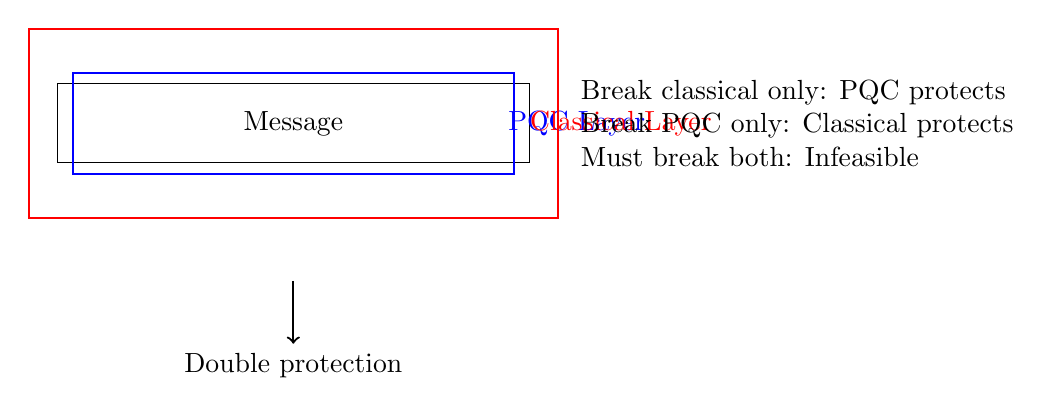
\begin{tikzpicture}[scale=0.8]
    % Nested encryption
    \node[draw, rectangle, minimum width=6cm, minimum height=1cm] (msg) at (0,0) {Message};

    \draw[thick, blue] (-3.5,-0.8) rectangle (3.5,0.8);
    \node[blue] at (4.5,0) {PQC Layer};

    \draw[thick, red] (-4.2,-1.5) rectangle (4.2,1.5);
    \node[red] at (5.2,0) {Classical Layer};

    % Arrows
    \draw[->, thick] (0,-2.5) -- (0,-3.5);
    \node[below] at (0,-3.5) {Double protection};

    % Attack scenarios
    \node[align=left] at (8,0) {
        Break classical only: PQC protects\\
        Break PQC only: Classical protects\\
        Must break both: Infeasible
    };
\end{tikzpicture}
\caption{Nested hybrid layers.  The message is protected by both a post-quantum and a classical cryptographic layer; security is maintained as long as at least one layer remains unbroken.}
\label{fig:ch13-hybrid-layers}
\end{figure}


\subsection{X.509 Hybrid Certificates}
\label{subsec:x509-hybrid}

Deploying hybrid signatures within the X.509 public-key infrastructure\index{X.509!hybrid certificates} requires encoding two public keys and two signatures into a single certificate.  Three strategies have been proposed:

\begin{enumerate}
\item \textbf{Dual-key certificate:} A single certificate carries both public keys and is signed with both CA keys.  The IETF draft \texttt{draft-ounsworth-pq-composite-sigs} defines composite OIDs for this approach.
\item \textbf{Catalyst certificate:} The classical certificate includes the PQC public key and signature in a non-critical X.509v3 extension.  Legacy clients ignore the extension; PQC-aware clients verify both.
\item \textbf{Paired certificates:} Two separate certificates---one classical, one PQC---are bound by a shared serial number.  The server sends both; the client verifies whichever it supports.
\end{enumerate}

The catalyst approach offers the best backward compatibility: existing TLS stacks parse the certificate without modification, while updated clients gain quantum resistance.  The cost is roughly $5$--$6$~KB of additional data per certificate (dominated by the ML-DSA public key and CA signature).


\subsection{Performance Impact}
\label{subsec:hybrid-performance}

\begin{table}[t]
\caption{Hybrid KEM overhead: X25519 + ML-KEM-768}
\label{tab:hybrid-overhead}
\begin{tabular}{p{3.5cm}p{2cm}p{2cm}p{2cm}p{2cm}}
\hline\noalign{\smallskip}
\textbf{Operation} & \textbf{X25519} & \textbf{ML-KEM-768} & \textbf{Hybrid} & \textbf{Factor} \\
\noalign{\smallskip}\svhline\noalign{\smallskip}
Key generation & 45\,\textmu s & 35\,\textmu s & 80\,\textmu s & 1.8$\times$ \\
Encapsulation   & 45\,\textmu s & 44\,\textmu s & 89\,\textmu s & 2.0$\times$ \\
Decapsulation   & 45\,\textmu s & 40\,\textmu s & 85\,\textmu s & 1.9$\times$ \\
Ciphertext size  & 32\,B & 1{,}088\,B & 1{,}120\,B & 35$\times$ \\
\noalign{\smallskip}\hline
\end{tabular}
\end{table}

The computational overhead of hybrid KEMs is modest ($< 2\times$), because ML-KEM operations are fast.  The dominant cost is \emph{bandwidth}: the combined ciphertext and public-key material adds roughly 2\,KB per handshake, which matters on constrained links but is negligible on broadband.


%% ================================================================
\section{TLS Migration}
\label{sec:tls-migration}

TLS~1.3 protects billions of HTTPS connections daily and is the highest-priority migration target.  Its clean key-exchange design---a single round-trip with ephemeral Diffie--Hellman---makes post-quantum integration relatively straightforward compared with older protocols.

\subsection{TLS 1.3 with Post-Quantum Key Exchange}
\label{subsec:tls13-pq}

TLS~1.3 negotiates key exchange via \emph{named groups}\index{TLS~1.3!named groups} advertised in the \texttt{supported\_groups} extension.  Adding a post-quantum or hybrid KEM requires:
\begin{enumerate}
\item Assigning a new named-group code point (e.g., \texttt{0x6399} for X25519Kyber768\index{X25519Kyber768}).
\item Extending buffer sizes: the \texttt{ClientHello} key-share grows from 32~bytes (X25519) to $\approx$\,1{,}216~bytes; the \texttt{ServerHello} encapsulation adds $\approx$\,1{,}088~bytes.
\item Combining the shared secrets via the TLS~1.3 key schedule: $\mathit{SS}_{\mathrm{hybrid}} = \mathrm{HKDF\text{-}Extract}(K_{\mathrm{X25519}} \| K_{\mathrm{ML\text{-}KEM}})$.
\end{enumerate}

Crucially, the handshake \emph{message count} does not change---the post-quantum material is embedded in the existing \texttt{key\_share} extension---so the protocol retains its 1-RTT structure.

\subsection{Chrome and Cloudflare Experiments}
\label{subsec:chrome-cloudflare}

\begin{example}[CECPQ2 and Beyond]
\label{ex:cecpq2}
\index{CECPQ2}
Google and Cloudflare have conducted the largest post-quantum TLS experiments to date:
\begin{itemize}
\item \textbf{2019:} CECPQ2 deployed hybrid ECDH + NTRU-HRSS in Chrome, covering $\sim$30\% of TLS connections to Google servers.  Median latency increase: 1\,ms.  User complaints: zero.
\item \textbf{2022:} Cloudflare switched to hybrid X25519 + Kyber-768, making PQC available across 20+ million websites.
\item \textbf{2023--2024:} Chrome enabled X25519Kyber768 by default.  By late 2024, over 10\% of all global HTTPS traffic used a post-quantum key exchange.
\end{itemize}
These experiments demonstrated that Internet-scale hybrid deployment is feasible with negligible user-facing impact.
\end{example}

\subsection{X25519Kyber768}
\label{subsec:x25519kyber768}

X25519Kyber768 (also known as \texttt{X25519MLKEM768} after the FIPS~203~\cite{FIPS203} renaming) is the first hybrid KEM deployed at scale.  It concatenates the 32-byte X25519 shared secret with the 32-byte ML-KEM-768 shared secret and feeds the 64-byte result into the TLS~1.3 HKDF key schedule.  The combined ciphertext is $32 + 1{,}088 = 1{,}120$~bytes---well within a single TCP segment, avoiding handshake fragmentation in most network conditions.


\subsection{Certificate Chain Sizes and Latency}
\label{subsec:cert-chain-sizes}

While key exchange adds $\sim$2\,KB, the larger concern is \emph{certificate chains}\index{certificate chain!PQC overhead}.  A three-certificate chain with ML-DSA-65 signatures grows from $\sim$3\,KB (RSA-2048) to $\sim$17\,KB, a 5.5$\times$ increase.

\begin{table}[t]
\caption{TLS handshake size and latency overhead}
\label{tab:tls-overhead}
\begin{tabular}{p{4cm}p{2.5cm}p{2.5cm}p{2.5cm}}
\hline\noalign{\smallskip}
\textbf{Component} & \textbf{Classical} & \textbf{PQC/Hybrid} & \textbf{Increase} \\
\noalign{\smallskip}\svhline\noalign{\smallskip}
Key exchange & 96\,B & 2{,}336\,B & 24$\times$ \\
Certificate chain (3 certs) & 3{,}150\,B & 17{,}235\,B & 5.5$\times$ \\
Total handshake & $\sim$3.5\,KB & $\sim$20\,KB & 5.7$\times$ \\
Median latency & baseline & +1.3\,ms & --- \\
95th-pct latency & baseline & +21\,ms & --- \\
\noalign{\smallskip}\hline
\end{tabular}
\end{table}

On desktop broadband, the extra latency is invisible.  On mobile networks with high round-trip times, the 95th-percentile overhead can reach 20--90\,ms, primarily due to TCP-level fragmentation and retransmission when the handshake exceeds the initial congestion window.  Session resumption via TLS~1.3 PSK mode avoids this cost entirely and becomes \emph{more important} in a post-quantum world.

\begin{svgraybox}
\textbf{The middlebox problem.}  Corporate firewalls and deep-packet-inspection appliances often impose hard limits on TLS record sizes (commonly 8\,KB or 16\,KB).  PQC certificate chains that exceed these limits are silently dropped, causing mysterious connection failures.  Early deployers report 2--6~weeks of debugging before identifying the root cause.  The fix is to fragment certificates across multiple TLS records or to use certificate compression (RFC~8879).
\end{svgraybox}


%% ================================================================
\section{Code Signing and Software Supply Chain}
\label{sec:code-signing}

Code signing\index{code signing} presents challenges distinct from TLS: signatures are verified \emph{years} after creation, backward compatibility with legacy verifiers is critical, and signature size directly affects software distribution costs.

\subsection{Firmware Updates}
\label{subsec:firmware}

Embedded devices---IoT sensors, medical implants, industrial controllers---verify firmware signatures using public keys burned into hardware at manufacture.  These keys may need to remain valid for 10--20~years, making them high-priority targets for ``harvest now, decrypt later'' attacks on confidentiality and, more critically, for future signature-forgery attacks on integrity.  A quantum adversary who can forge a firmware signature can push malicious updates to every device in the fleet.

Stateful hash-based signature schemes (LMS\index{LMS}, XMSS\index{XMSS}), standardized in NIST~SP~800-208, are attractive for firmware signing because their security rests purely on hash-function properties and they produce compact signatures ($\sim$2.5\,KB for LMS with $H=20$).  The main operational burden is state management: each private key must track which one-time keys have been used, and reuse is catastrophic.  For CA root keys that sign infrequently, this burden is manageable.

\subsection{Package Managers and Repository Signing}
\label{subsec:package-managers}

Software supply chains (npm, PyPI, apt, Homebrew) sign repository metadata and individual packages.  A single compromised signing key can inject malicious code into millions of systems.  Migration considerations include:
\begin{itemize}
\item \textbf{Dual signatures:} Repositories can distribute both classical and PQC signatures in parallel.  Clients verify whichever their toolchain supports.
\item \textbf{Transparency logs:} Systems like Sigstore already decouple signatures from distribution, easing algorithm transitions.
\item \textbf{Threshold signing:} Multi-party signing ceremonies (common for root keys) must be updated to use PQC-compatible threshold protocols.
\end{itemize}

\subsection{The Signature Size Challenge}
\label{subsec:sig-size-challenge}

\begin{table}[t]
\caption{Signature sizes for code-signing candidates}
\label{tab:codesign-sizes}
\begin{tabular}{p{3.5cm}p{2.5cm}p{2.5cm}p{3cm}}
\hline\noalign{\smallskip}
\textbf{Scheme} & \textbf{Signature} & \textbf{Public key} & \textbf{Security basis} \\
\noalign{\smallskip}\svhline\noalign{\smallskip}
RSA-2048 & 256\,B & 294\,B & Factoring \\
ECDSA-P256 & 64\,B & 64\,B & ECDLP \\
ML-DSA-65 & 3{,}309\,B & 1{,}952\,B & Module-LWE \\
SLH-DSA-128s & 7{,}856\,B & 32\,B & Hash functions \\
LMS ($H{=}20$) & 2{,}508\,B & 56\,B & Hash functions \\
\noalign{\smallskip}\hline
\end{tabular}
\end{table}

For a typical software update containing 1{,}000--10{,}000 signed files, switching from RSA-2048 to ML-DSA-65 increases total signature overhead from $\sim$250\,KB to $\sim$3.3\,MB per update.  SLH-DSA offers the advantage of minimal public-key size and conservative, hash-only security assumptions, but its signatures are 2--3$\times$ larger than ML-DSA.  The practical choice depends on whether the deployment is bandwidth-constrained (favour ML-DSA) or demands maximal cryptographic conservatism (favour SLH-DSA or LMS for root keys).

The signature-size tension is annoying for software distribution; for blockchain systems, where every byte is replicated across thousands of nodes and stored forever, it becomes an existential design constraint.

%% ================================================================
\section{Blockchain and Cryptocurrencies}
\label{sec:blockchain}

Blockchain systems face a ``perfect storm'' of post-quantum migration challenges: immutable transaction histories, size-sensitive economics, decentralized governance, and catastrophic failure modes.  Until recently, the standard consolation was that breaking ECDSA-256 would require millions of physical qubits and hours to days of continuous quantum computation---a threshold that seemed comfortably distant.  That consolation has evaporated.

\subsection{ECDSA Vulnerability: New Resource Estimates}
\label{subsec:ecdsa-vulnerability}

Bitcoin, Ethereum, and most cryptocurrencies derive address security from ECDSA over the \texttt{secp256k1} curve.  Shor's algorithm\index{Shor's algorithm!ECDSA} recovers private keys from public keys in polynomial time, and the practical resource estimates for carrying out such an attack have improved dramatically.  Babbush, Zalcman, Gidney et~al.~\cite{BabbushZalcmanGidney2026}, in a collaboration spanning Google Quantum AI, the Ethereum Foundation, UC~Berkeley, and Stanford, demonstrated that ECC-256 can be broken in \emph{minutes}---not hours, not days---using fewer than 500{,}000 physical qubits on a superconducting architecture.  This is roughly the scale that multiple hardware roadmaps target within the next decade.

The shift from ``years with millions of qubits'' to ``minutes with fewer than half a million'' is not incremental; it changes the character of the threat.  A multi-hour attack allows defenders to detect anomalous quantum activity and respond; a multi-minute attack does not.  The window between vulnerability and exploitation has collapsed to the timescale of a single blockchain confirmation interval.

\subsection{Attack Taxonomy}
\label{subsec:attack-taxonomy}

\index{blockchain!attack taxonomy}
The resource estimates from Babbush et~al.~\cite{BabbushZalcmanGidney2026} sharpen the threat model into three distinct attack classes, each with different hardware requirements and different consequences.

\paragraph{On-spend attacks.}  The adversary monitors the mempool for pending transactions that reveal a public key, extracts the private key via Shor's algorithm, and submits a competing transaction redirecting the funds---all before the original transaction is confirmed in a block.  This attack requires a \emph{fast-clock} CRQC: the quantum computation must complete within the confirmation window, typically 10~minutes for Bitcoin and 12~seconds for Ethereum.  The new sub-minute resource estimates mean that superconducting and photonic architectures are fast enough for on-spend attacks against both networks.  The attack is surgical: it targets individual transactions in real time and leaves no trace until the victim's funds vanish.

\paragraph{At-rest attacks.}  Coins held in addresses where the public key was previously exposed---through a past spend, through address reuse, or through legacy pay-to-public-key (P2PK) scripts---are vulnerable to \emph{leisurely} quantum attack.  The adversary need not race a confirmation timer; the public key is already on-chain, visible to anyone.  Crucially, at-rest attacks do not require fast-clock hardware.  Slow-clock CRQCs based on neutral atoms or trapped ions, which may reach cryptographic relevance on a different timeline than superconducting machines, suffice.  This broadens the set of potential attackers: a neutral-atom machine that takes hours to break a single key is useless for on-spend attacks but perfectly adequate for draining a dormant wallet.

\paragraph{On-setup attacks.}  The adversary compromises the key-generation process itself, either by attacking the randomness source or by intercepting the public key at creation time and pre-computing the private key before the address is ever funded.  On-setup attacks are the least discussed but potentially the most insidious, because the compromise is invisible until the adversary chooses to act.

This taxonomy matters because it determines which defences are effective against which threats.  Commit-reveal schemes and shorter confirmation windows mitigate on-spend attacks but do nothing for at-rest exposure.  Conversely, address-migration campaigns address at-rest risk but cannot protect a transaction in flight.  A comprehensive defence must address all three classes.

\subsection{Migration Challenges}
\label{subsec:blockchain-migration}

The ECDSA vulnerability is clear enough; what makes blockchain migration uniquely difficult is that every proposed remedy collides with a core design property.

Consider immutability first.  The blockchain's defining feature---that no past record can be altered---becomes a liability when past records contain quantum-vulnerable signatures.  Historical ECDSA signatures cannot be replaced, only supplemented with new PQC protections going forward.  This stands in sharp contrast to a TLS deployment, where rotating to new certificates immediately protects all future sessions and the old certificates simply expire.

Transaction size compounds the problem.  Replacing ECDSA ($\sim$72\,B per signature) with ML-DSA-44 ($\sim$2{,}420\,B) inflates a simple Bitcoin transaction from $\sim$250\,B to $\sim$3{,}500\,B---a 14$\times$ increase.  Block capacity drops from $\sim$4{,}000 to $\sim$285~transactions, fees rise proportionally, and full-node storage grows from $\sim$50\,GB/year to $\sim$700\,GB/year.  In a system where every full node stores the complete history, this is not merely a bandwidth cost; it reshapes the economics of participation.

Governance adds a further constraint.  Any signature-scheme change requires a hard fork or, at minimum, a soft fork with broad community agreement.  In decentralized networks, achieving such agreement can take years---the Bitcoin block-size debate (2015--2017) is a cautionary precedent.

Finally, address migration demands active participation from every user.  Funds must be moved to quantum-safe addresses through on-chain transactions, which means every wallet holder must act.  The next subsection quantifies how large the exposure actually is.

Figure~\ref{fig:ch14-blockchain-immutability} captures the core dilemma: the blockchain's immutability---its defining strength---means that historical ECDSA signatures cannot be replaced, only supplemented, while a quantum attacker who can forge those signatures threatens every block in the chain.

\begin{figure}[t]
\centering
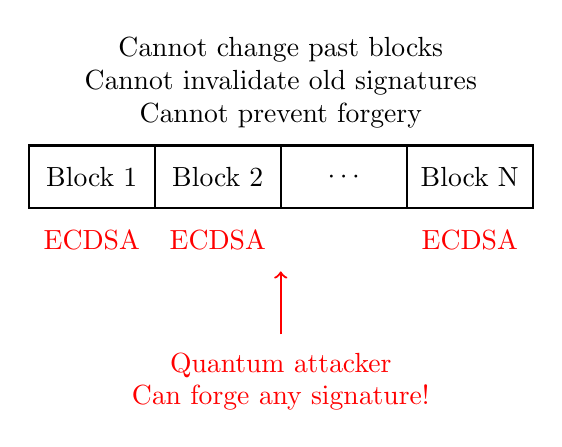
\begin{tikzpicture}[scale=0.8]
    % Blockchain
    \draw[thick] (0,0) rectangle (2,1);
    \node at (1,0.5) {Block 1};
    \draw[thick] (2,0) rectangle (4,1);
    \node at (3,0.5) {Block 2};
    \draw[thick] (4,0) rectangle (6,1);
    \node at (5,0.5) {$\cdots$};
    \draw[thick] (6,0) rectangle (8,1);
    \node at (7,0.5) {Block N};

    % Signatures
    \node[red] at (1,-0.5) {ECDSA};
    \node[red] at (3,-0.5) {ECDSA};
    \node[red] at (7,-0.5) {ECDSA};

    % Quantum attack
    \draw[thick, red, ->] (4,-2) -- (4,-1);
    \node[red] at (4,-2.5) {Quantum attacker};
    \node[red] at (4,-3) {Can forge any signature!};

    % Problem
    \node[align=center] at (4,2) {Cannot change past blocks\\Cannot invalidate old signatures\\Cannot prevent forgery};
\end{tikzpicture}
\caption{Blockchain immutability versus PQC migration: past blocks are secured by ECDSA signatures that cannot be replaced, yet a quantum attacker could forge any of them---making migration nearly impossible for historical data.}
\label{fig:ch14-blockchain-immutability}
\end{figure}

\subsection{Dormant Assets and Frozen Funds}
\label{subsec:frozen-funds}

\index{frozen funds risk}
\index{dormant assets}
The at-rest attack class is not a theoretical curiosity; its scope is enormous.  Babbush et~al.~\cite{BabbushZalcmanGidney2026} estimate that 1.7~million~BTC are locked in early pay-to-public-key (P2PK) scripts whose public keys sit permanently on-chain, exposed and waiting.  These are among the oldest coins in the network---many date from the Satoshi era and the first two years of mining---and they have never been moved.  When address reuse is included (users who inadvertently revealed their public keys by spending from the same address more than once), the total quantum-vulnerable dormant supply may reach 2.3~million~BTC.  At any plausible valuation, this constitutes a systemic-scale exposure.

The community has proposed several mitigation strategies for these dormant assets, none of them painless.  Each trades one kind of harm for another.

The first option is to \emph{do nothing}: accept the risk, and let quantum-vulnerable coins be stolen when a CRQC arrives.  This is the path of least governance friction but the greatest economic damage.  It effectively transfers wealth from early adopters (and lost-key holders) to whoever builds or controls the first CRQC.

The second is \emph{burn}: the network permanently destroys coins in quantum-vulnerable addresses after a deadline, removing them from the supply.  This eliminates the theft vector but also eliminates the assets, which is indistinguishable from confiscation for any holder who was merely inactive rather than absent.

The third is the \emph{hourglass deadline}: after a community-agreed date, the network rejects transactions from addresses that have not migrated to PQC keys.  Funds are not destroyed but are frozen indefinitely.  This protects the system from quantum theft while preserving the theoretical possibility that holders could reclaim their coins if a future protocol change permits it.  The measure is politically explosive; it amounts to a collective decision to sacrifice some holders' access for the security of the whole, a trade-off with no precedent in Bitcoin's history.

A fourth proposal is the \emph{bad sidechain}: a parallel chain secured by PQC signatures that accepts bridged assets from the main chain.  Users lock funds on the classical chain and receive equivalent tokens on the sidechain, migrating at their own pace without requiring a hard fork.  The approach is technically sound but adds operational complexity and splits network effects.

The fifth and most creative proposal is \emph{digital salvage}~\cite{BabbushZalcmanGidney2026}---a legal framework analogous to maritime salvage law, under which dormant quantum-vulnerable coins could be claimed by parties who invest in securing or migrating them, subject to a duty to compensate the original owner if they later resurface.  Maritime law has centuries of precedent for handling property that is lost, abandoned, or in imminent peril; the argument is that digital assets in quantum-vulnerable addresses fit the same pattern.  Whether courts or protocol governance would accept this analogy remains entirely open, but the proposal illustrates how far the dormant-asset problem reaches beyond cryptography and into law and political economy.

For any of these paths, the commit-reveal technique offers a partial shield for \emph{future} transactions.  Users commit a hash of a PQC public key to the blockchain now, then reveal the actual key only when spending.  Because the quantum-vulnerable classical public key never enters the mempool, a CRQC operator cannot execute an on-spend attack.  The limitation is clear---commit-reveal does nothing for the 1.7--2.3~million BTC whose public keys were exposed long ago.

\subsection{Ethereum: Deeper Exposure}
\label{subsec:ethereum-exposure}

\index{Ethereum!quantum vulnerability}
If Bitcoin's vulnerability is severe, Ethereum's is structural.  Babbush et~al.~\cite{BabbushZalcmanGidney2026} argue that Ethereum is \emph{more exposed} than Bitcoin across several dimensions, each rooted in a design decision that was reasonable in a pre-quantum world.

The most fundamental difference is the account model.  Bitcoin uses a UTXO model in which public keys need not be revealed until spending; Ethereum's account model exposes every externally owned account's (EOA) public key permanently on-chain from the first outgoing transaction.  Every active Ethereum address is therefore vulnerable to at-rest attack from the moment it sends its first transaction.  There is no hash-based address abstraction to hide behind.

Proof-of-Stake introduces a second attack surface.  Ethereum validators stake 32~ETH and sign attestations and block proposals with keys that are permanently visible to the network.  A CRQC operator who can forge validator signatures can execute slashing attacks, produce conflicting attestations, or seize control of the consensus layer.  Unlike a stolen user key---which harms one account---a compromised validator key undermines the integrity of the chain itself.

Smart-contract governance adds a third dimension.  Many high-value protocols (DAOs, DeFi lending pools, multi-signature treasuries) gate critical operations on ECDSA-signed messages.  A quantum adversary who can forge these signatures can drain treasuries, modify governance parameters, or upgrade contract logic unilaterally.  The damage is not limited to the attacker's own transactions; it extends to every contract that trusts a quantum-vulnerable signature.

Finally, Ethereum's Data Availability Sampling (DAS) layer, central to the rollup-centric scaling roadmap, relies on cryptographic commitments that must remain binding.  If the underlying elliptic-curve assumptions fall, the data-availability guarantees collapse, and with them the security model of every Layer~2 rollup built on top.

Ethereum's account-abstraction roadmap (EIP-4337 and successors) offers the most credible migration path.  By decoupling signature verification from the protocol layer, smart-contract wallets can adopt PQC signature schemes without a hard fork.  The planned sequence is: enable smart-contract wallets (2024--2025), support hybrid signatures (2025--2027), incentivize migration via gas discounts (2027--2029), and disable raw ECDSA for new transactions (2030+).  This is an ambitious and well-structured plan, but it still requires years of coordinated effort, and it does nothing for the vast stock of EOAs that have already exposed their public keys.

\subsection{Tokenization and Systemic Risk}
\label{subsec:tokenization-risk}

\index{tokenization!quantum risk}
The blockchain quantum risk extends well beyond cryptocurrency speculation.  Real-world asset (RWA) tokenization---the representation of equities, bonds, real estate, and commodities as on-chain tokens---is projected to exceed 16~trillion~USD by 2030~\cite{BabbushZalcmanGidney2026}.  This is not a niche market; it is a substantial fraction of the global financial system migrating onto infrastructure that, as of this writing, remains quantum-vulnerable.

The ``too big to fail'' threshold is approaching.  When trillions of dollars in tokenized assets sit on chains secured by ECDSA, the quantum threat ceases to be a concern for cryptocurrency enthusiasts and becomes a systemic financial risk.  Regulators, central banks, and institutional investors who might otherwise ignore the blockchain migration debate will be compelled to engage once their own balance sheets depend on elliptic-curve security.

This convergence of quantum computing timelines and tokenization growth creates a hard constraint: the blockchain ecosystem must complete its PQC migration before the tokenized asset base reaches a scale at which a quantum breach triggers cascading financial contagion.  The migration window is not defined solely by qubit roadmaps; it is also defined by the pace at which traditional finance moves on-chain.

\subsection{Migration Urgency}
\label{subsec:blockchain-urgency}

\index{blockchain!migration urgency}
The overall picture, as Babbush et~al.~\cite{BabbushZalcmanGidney2026} conclude, is neither hopeless nor comfortable.  There \emph{is} time to migrate---the sub-500K-qubit machines needed for real-time ECDSA breaks do not yet exist, and the engineering path from current hardware to that threshold is nontrivial.  But the margin for error is increasingly narrow.  The resource estimates have improved faster than the migration efforts, and every year of delay narrows the gap between ``when we can be attacked'' and ``when we will be ready.''

Blockchain migration illustrates, in extreme form, the tension between technical necessity and organizational inertia.  The next section generalizes this tension into a structured roadmap applicable to any organization, blockchain or otherwise.


%% ================================================================
\section{Organizational Roadmap}
\label{sec:roadmap}

The preceding sections examined specific migration targets---TLS, code signing, blockchain---each with its own technical constraints.  But even perfect technical solutions fail without organizational execution.  Organizations must run a structured migration program that touches procurement, engineering, compliance, and operations in coordinated sequence.  The six-phase roadmap below distills guidance from NIST~SP~1800-38, the NSA's CNSA~2.0 advisory, and European agency recommendations into a practical framework.  It is ordered by dependency: each phase produces the inputs the next phase requires.

\subsection{Phase 1: Cryptographic Inventory}
\label{subsec:phase-inventory}

\index{cryptographic inventory}
No migration can succeed without knowing what must be moved.  The first phase is a comprehensive discovery of every use of public-key cryptography across the organization: TLS certificates, code-signing keys, VPN configurations, SSH keys, API tokens, hardware security modules, embedded-device firmware, and third-party dependencies.  The analogy to physical logistics is apt---before relocating a warehouse, one inventories every pallet; skipping this step guarantees that critical items are left behind.

Automated scanning tools (Venafi, Keyfactor, or open-source \texttt{cbom} generators) provide a starting point, but they rarely find everything.  Manual review is essential, particularly for shadow IT and legacy systems maintained by teams outside central security.  A typical medium enterprise discovers that 40--50\% of its cryptographic assets were unknown to the security team before the inventory---a sobering figure that explains why so many migrations stall in later phases.

With a complete inventory in hand, the organization can move to risk assessment: not all assets face the same quantum exposure, and treating them uniformly wastes resources.

\subsection{Phase 2: Risk Assessment}
\label{subsec:phase-risk}

The inventory tells us \emph{what} the organization has; risk assessment determines \emph{what is at stake}.  Each asset is classified along two dimensions: \emph{data sensitivity lifetime}---how long must the data remain confidential or its signatures remain trusted?---and \emph{migration difficulty}---how hard is it to change the algorithm?  Assets that score high on both dimensions (long-lived secrets protected by deeply embedded cryptography) demand immediate attention; ephemeral session keys on modern, patchable servers can wait.

\begin{table}[t]
\caption{Risk classification matrix}
\label{tab:risk-matrix}
\begin{tabular}{p{3.5cm}p{2.5cm}p{2.5cm}p{3cm}}
\hline\noalign{\smallskip}
\textbf{Data category} & \textbf{Lifetime} & \textbf{Risk level} & \textbf{Action} \\
\noalign{\smallskip}\svhline\noalign{\smallskip}
Government / military & 25--50 years & Critical & Immediate \\
Healthcare records & 50--100 years & Critical & Immediate \\
Financial records & 7--10 years & High & By 2027 \\
Trade secrets / IP & 10--20 years & High & By 2027 \\
Personal data (GDPR) & Lifetime & Medium & By 2029 \\
Ephemeral session keys & Hours & Low & By 2031 \\
\noalign{\smallskip}\hline
\end{tabular}
\end{table}

\subsection{Phase 3: Prioritize}
\label{subsec:phase-prioritize}

Risk assessment produces a ranked list; prioritization turns that list into a work plan.  The principle is straightforward---start with the highest-risk, longest-lived data---but the practical ordering requires judgment about dependencies and organizational capacity.

VPN tunnels and TLS sessions protecting classified or regulated data typically top the list, because they are actively exposed to harvest-now-decrypt-later attacks and Mosca's inequality (Sect.~\ref{subsec:mosca}) is already violated for multi-decade secrets.  Root CA and code-signing keys follow closely: they are long-lived, their compromise has cascading impact, and their migration is largely independent of application-layer changes.  Data-at-rest encryption keys for archives with multi-decade retention come next, followed by customer-facing web services, which benefit from well-understood migration paths (Sect.~\ref{sec:tls-migration}) and high public visibility.

The prioritized list feeds directly into the testing phase, where each migration path is validated before it touches production traffic.

\subsection{Phase 4: Test}
\label{subsec:phase-test}

Before any PQC algorithm touches production traffic, it must survive contact with reality.  Hybrid modes are deployed first in staging and pre-production environments, where failures are cheap and reversible.

Testing spans several dimensions.  Functional correctness is the baseline: do the hybrid handshakes complete, and do the resulting session keys match on both sides?  Latency and throughput under load reveal whether the larger key material degrades performance beyond acceptable thresholds---the middlebox problem described in Sect.~\ref{subsec:cert-chain-sizes} is routinely discovered at this stage.  Interoperability testing with legacy clients and middleboxes is critical, because a migration that breaks 2\% of connections will be rolled back before it protects anyone.  Failure-mode behavior must be explicitly validated: does the system fall back gracefully to classical-only when the PQC component is unavailable, or does it fail hard?  Finally, key and certificate lifecycle operations---renewal, revocation, rotation---must work end-to-end, because a migration that cannot maintain itself is a migration that will decay.

Testing failures are not setbacks; they are the point.  Every incompatibility caught here is one that does not become a 2\,AM incident in production.

\subsection{Phase 5: Deploy}
\label{subsec:phase-deploy}

Deployment follows the same graduated-rollout discipline used for any high-risk infrastructure change---the difference is that the stakes include long-term cryptographic exposure, not just transient outages.

The rollout begins with a canary deployment to roughly 1\% of traffic, chosen to include a representative mix of client populations.  At this scale, gross incompatibilities surface---broken middleboxes, misconfigured load balancers, clients that choke on larger handshakes---without affecting the majority of users.  Once the canary is stable, traffic shifts to 10\% (early adopters), where performance under realistic load is validated against the baselines established in testing.  The move to 50\% exercises the system at scale: tail latencies, connection-retry rates, and certificate-chain failures that appear only under heavy load become visible.  Full deployment at 100\% completes the migration, but the classical algorithm is not removed---it remains available as a fallback until the organization is confident that every client ecosystem has adapted.

Throughout each stage, monitoring dashboards track handshake failure rates, latency distributions, and certificate-validation errors.  Any regression beyond predefined thresholds triggers an automatic rollback to the previous traffic split.  Figure~\ref{fig:ch14-canary-deploy} illustrates this graduated rollout, with the rollback path that makes each stage reversible.

\begin{figure}[t]
\centering
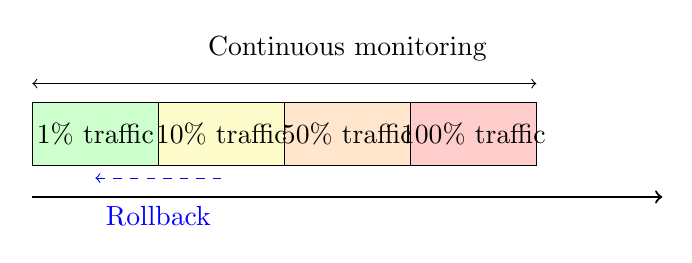
\begin{tikzpicture}[scale=0.8]
    % Timeline
    \draw[thick, ->] (0,0) -- (10,0);

    % Phases
    \draw[fill=green!20] (0,0.5) rectangle (2,1.5);
    \node at (1,1) {1\% traffic};

    \draw[fill=yellow!20] (2,0.5) rectangle (4,1.5);
    \node at (3,1) {10\% traffic};

    \draw[fill=orange!20] (4,0.5) rectangle (6,1.5);
    \node at (5,1) {50\% traffic};

    \draw[fill=red!20] (6,0.5) rectangle (8,1.5);
    \node at (7,1) {100\% traffic};

    % Monitoring
    \node[above] at (5,2) {Continuous monitoring};
    \draw[<->] (0,1.8) -- (8,1.8);

    % Rollback
    \draw[->, dashed, blue] (3,0.3) -- (1,0.3);
    \node[below, blue] at (2,0) {Rollback};
\end{tikzpicture}
\caption{Canary deployment for PQC migration: traffic is shifted in graduated stages with continuous monitoring, and any regression triggers an automatic rollback to the previous stage.}
\label{fig:ch14-canary-deploy}
\end{figure}

\subsection{Phase 6: Verify and Maintain}
\label{subsec:phase-verify}

A migration that declares victory at 100\% deployment and moves on has failed.  Cryptographic infrastructure is a living system: new services are provisioned, dependencies are updated, developers under deadline pressure reach for the defaults their frameworks provide---and those defaults may still be classical.

Continuous compliance therefore requires several ongoing disciplines.  Monitoring detects \emph{algorithm drift}, where newly deployed services silently revert to classical-only configurations.  Automated alerting fires when certificates or keys use deprecated algorithms, catching regressions before they reach production.  Periodic reassessment accounts for advances in cryptanalysis: a parameter set considered safe in 2026 may need revision by 2030 as lattice-reduction techniques improve.

The deepest lesson of this phase is the importance of \emph{crypto-agility}\index{crypto-agility}---the architectural ability to swap algorithms without redesigning protocols or redeploying hardware.  Crypto-agility is not a feature to add later; it is a design principle that must be embedded from Phase~1 onward.  Organizations that achieve it will navigate not only the post-quantum transition but every subsequent cryptographic migration with far less friction.

The CNSA~2.0 timeline and European guidance that follow provide the external deadlines against which these six phases must be scheduled.

\subsection{CNSA 2.0 Timeline}
\label{subsec:cnsa20}

\index{CNSA 2.0}
The six phases above describe \emph{how} to migrate; the CNSA~2.0 timeline specifies \emph{when}.  The NSA's Commercial National Security Algorithm Suite~2.0 sets mandatory deadlines for U.S.\ national-security systems, and these deadlines increasingly serve as de facto benchmarks for the private sector as well:

\begin{table}[t]
\caption{CNSA 2.0 transition deadlines (NSA, 2022)}
\label{tab:cnsa20}
\begin{tabular}{p{4.5cm}p{3.5cm}p{3.5cm}}
\hline\noalign{\smallskip}
\textbf{Use case} & \textbf{Algorithm} & \textbf{Deadline} \\
\noalign{\smallskip}\svhline\noalign{\smallskip}
Software / firmware signing & CNSA~2.0 exclusive & 2025 \\
Web servers / cloud services & CNSA~2.0 preferred & 2025 \\
Traditional networking (VPN, routers) & CNSA~2.0 preferred & 2026 \\
Operating systems & CNSA~2.0 support & 2027 \\
Custom / embedded applications & CNSA~2.0 exclusive & 2030 \\
Legacy infrastructure & CNSA~2.0 exclusive & 2033 \\
\noalign{\smallskip}\hline
\end{tabular}
\end{table}

\subsection{European Guidance}
\label{subsec:eu-guidance}

CNSA~2.0 is a U.S.-centric framework; European agencies set their own timelines, informed by different threat models and regulatory structures, but converging on similar urgency.

ANSSI (France) recommends hybrid modes as mandatory during the transition period and requires PQC for new systems handling classified data from 2025 onward.  Notably, ANSSI explicitly endorses FrodoKEM alongside ML-KEM as a conservative alternative for high-security applications---reflecting a preference for schemes with stronger theoretical security reductions, even at a performance cost.  BSI (Germany) recommends beginning migration planning immediately, with hybrid deployments by 2025 and full PQC by 2030; BSI requires a ``defence in depth'' approach combining lattice-based and hash-based schemes, ensuring that no single cryptanalytic breakthrough compromises the entire infrastructure.  At the EU level, ENISA published a post-quantum roadmap in 2022 urging member states to conduct cryptographic inventories by 2025 and complete critical-infrastructure migration by 2030.

The convergence across these agencies---American, French, German, European---is striking.  Despite differing institutional cultures and threat priorities, all place the start of serious migration activity no later than 2025 and demand completion for critical systems by 2030.  Whether these deadlines are achievable depends on the timeline pressures we examine next.


%% ================================================================
\section{Timeline and Urgency}
\label{sec:timeline}

The roadmap and regulatory deadlines of the previous section raise an obvious question: how late is too late?  The answer depends not on policy but on arithmetic---a simple inequality that formalizes the harvest-now-decrypt-later threat into a planning tool.

\subsection{Mosca's Inequality}
\label{subsec:mosca}

\index{Mosca's inequality}
Michele Mosca formalized the urgency of post-quantum migration with a simple but powerful inequality:

\begin{definition}[Mosca's Inequality]
\label{def:mosca}
Let:
\begin{itemize}
\item $x$ = the number of years the data must remain secure,
\item $y$ = the number of years needed to migrate the system to PQC,
\item $z$ = the number of years until a CRQC exists.
\end{itemize}
If $x + y > z$, then the data is \emph{already at risk today}, because an adversary can harvest ciphertext now and decrypt it once a CRQC is available before the confidentiality requirement expires.
\end{definition}

\begin{example}[Applying Mosca's Inequality]
\label{ex:mosca-hospital}
A hospital system stores patient records that must remain confidential for 50~years ($x = 50$).  Their IT department estimates that a full cryptographic migration will take 5~years ($y = 5$).  Assuming a CRQC arrives by 2035 ($z = 2035 - 2026 = 9$), we have $x + y = 55 \gg 9 = z$.  The inequality has been violated for decades: any patient record encrypted before 2026 with a classical algorithm is exposed to a harvest-now-decrypt-later attack.
\end{example}

The uncomfortable implication: for any data with a multi-decade confidentiality requirement, migration should have started years ago.  Figure~\ref{fig:ch13-migration-timeline} plots projected quantum capability against the cryptographic thresholds for current algorithms, making the shrinking migration window visually concrete.

\begin{figure}[t]
\centering
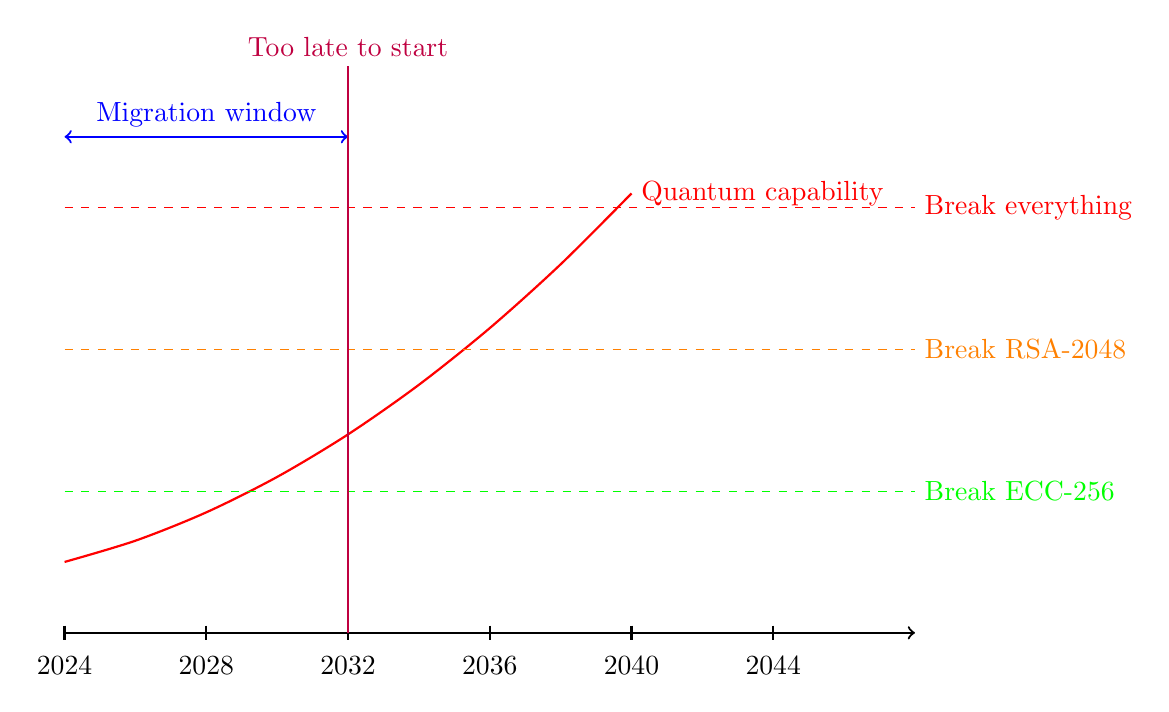
\begin{tikzpicture}[scale=0.9]
    % Timeline
    \draw[thick, ->] (0,0) -- (12,0);
    \foreach \x/\year in {0/2024, 2/2028, 4/2032, 6/2036, 8/2040, 10/2044} {
        \draw[thick] (\x,0.1) -- (\x,-0.1);
        \node[below] at (\x,-0.2) {\year};
    }

    % Quantum development
    \draw[thick, red] plot[smooth] coordinates {
        (0,1) (1,1.3) (2,1.7) (3,2.2) (4,2.8) (5,3.5) (6,4.3) (7,5.2) (8,6.2)
    };
    \node[red, right] at (8,6.2) {Quantum capability};

    % Threat levels
    \draw[dashed, green] (0,2) -- (12,2);
    \node[green, right] at (12,2) {Break ECC-256};

    \draw[dashed, orange] (0,4) -- (12,4);
    \node[orange, right] at (12,4) {Break RSA-2048};

    \draw[dashed, red] (0,6) -- (12,6);
    \node[red, right] at (12,6) {Break everything};

    % Key events
    \draw[thick, blue, <->] (0,7) -- (4,7);
    \node[blue, above] at (2,7) {Migration window};

    \draw[thick, purple] (4,0) -- (4,8);
    \node[purple, above] at (4,8) {Too late to start};
\end{tikzpicture}
\caption{Projected quantum capability versus classical cryptographic thresholds.  The migration window closes once quantum hardware crosses the first dashed threshold; organisations that have not begun transitioning by that point face irreversible exposure.}
\label{fig:ch13-migration-timeline}
\end{figure}

\subsection{Sector-Specific Deadlines}
\label{subsec:sector-deadlines}

Mosca's inequality is most useful when applied to concrete sectors, because different industries face radically different values of $x$, $y$, and~$z$:

\begin{table}[t]
\caption{Sector-specific Mosca analysis (assuming CRQC by 2035)}
\label{tab:sector-mosca}
\begin{tabular}{p{3cm}p{1.5cm}p{1.5cm}p{1.5cm}p{3.5cm}}
\hline\noalign{\smallskip}
\textbf{Sector} & $x$ (yr) & $y$ (yr) & $x+y$ & \textbf{Must start by} \\
\noalign{\smallskip}\svhline\noalign{\smallskip}
Intelligence & 50 & 8 & 58 & Already overdue \\
Healthcare & 50 & 5 & 55 & Already overdue \\
Finance & 10 & 4 & 14 & 2026 \\
Telecoms & 5 & 3 & 8 & 2027 \\
Retail / web & 2 & 2 & 4 & 2031 \\
\noalign{\smallskip}\hline
\end{tabular}
\end{table}

\subsection{Cost of Delay}
\label{subsec:cost-delay}

Delaying migration incurs compounding costs:
\begin{enumerate}
\item \textbf{Harvest-now exposure grows daily.}  Every additional day of classical-only encryption adds one more day of ciphertext to the adversary's stockpile.
\item \textbf{Technical debt accumulates.}  New systems deployed today without PQC support become tomorrow's ``legacy infrastructure''---the most expensive category to migrate.
\item \textbf{Talent scarcity.}  PQC expertise is limited.  Organizations that wait will compete for the same engineers during a compressed timeline, driving up costs.
\item \textbf{Regulatory risk.}  Once mandates like CNSA~2.0 take effect, non-compliant systems face operational restrictions or loss of certification.
\end{enumerate}

\begin{svgraybox}
\textbf{Lessons from previous cryptographic migrations.}
The AES transition (2001--2010) succeeded because it offered a drop-in replacement with better performance.  The IPv6 transition (1998--present, still incomplete) stalled because it required infrastructure changes with no immediate benefit.  PQC migration resembles IPv6 more than AES: the threat is not yet tangible, the changes are invasive, and the performance trade-offs are unfavorable.  Without deliberate urgency, a 20-year transition is a realistic worst case.
\end{svgraybox}


%% ================================================================
\section{Case Studies}
\label{sec:case-studies}

The six-phase roadmap, the regulatory deadlines, and the cost-of-delay analysis are abstractions until they collide with organisational reality.  Two early adopters---one in finance, one in government---illustrate how different threat models and institutional constraints shape the migration path.  Neither organisation is named, but the details are drawn from published deployment reports and direct consultation.

\subsection{A Major Financial Institution: Phased Hybrid Migration}
\label{subsec:case-finance}

\index{case study!financial institution}
A large international bank confronted the PQC transition with a straightforward threat model: high-value transactions and long-lived customer records protected by TLS, code-signing, and HSM-bound keys.  Regulatory pressure from multiple jurisdictions (CNSA~2.0 in the U.S., BSI guidance in Europe) compressed the timeline.  The bank chose a hybrid migration strategy---classical plus post-quantum in parallel---executed across four phases:

\begin{enumerate}
\item \textbf{Phase~1 (2024):} Internal systems and employee access.  VPN tunnels, internal certificate authorities, and developer code-signing keys were migrated to hybrid (X25519 + ML-KEM-768 for key exchange, RSA-2048 + ML-DSA-65 for signatures).  These systems had controlled client populations and could tolerate compatibility issues.
\item \textbf{Phase~2 (2025):} Customer-facing applications.  Online banking, mobile apps, and API gateways adopted hybrid TLS, using the X25519Kyber768 key exchange described in Sect.~\ref{subsec:x25519kyber768}.  A canary deployment at 1\% traffic (Sect.~\ref{subsec:phase-deploy}) caught three middlebox incompatibilities before wider rollout.
\item \textbf{Phase~3 (2026):} Inter-bank communication protocols.  SWIFT messaging and inter-bank settlement channels required coordination with counterparties---the hardest phase, because the bank could not unilaterally upgrade a bilateral protocol.
\item \textbf{Phase~4 (2027):} Legacy system integration.  Mainframe-based transaction processors and embedded HSMs with 10--15~year hardware refresh cycles---the ``long tail'' that every migration encounters.
\end{enumerate}

The bank encountered several obstacles that the six-phase roadmap anticipated but could not fully prepare for.  Regulatory approval for new cryptographic methods took longer than expected: two jurisdictions required independent validation of the hybrid construction before permitting its use for regulated transactions.  Performance impact on high-frequency trading systems was measurable---the larger ML-KEM ciphertexts increased TLS handshake latency by 15--20\%, triggering latency-budget reviews.  Integration with third-party vendors proved difficult when those vendors had not begun their own PQC migration.  Staff training and certification requirements consumed more calendar time than the technical work itself.

The lessons distilled from this deployment are worth stating plainly: start with low-risk internal systems to build operational experience before touching customer-facing infrastructure; engage regulators early, because cryptographic-method approval is a serial dependency that cannot be parallelised with engineering; invest in testing infrastructure before it is needed, not after the first production incident; and plan for timelines 50--100\% longer than initial estimates, because every phase reveals dependencies that were invisible during planning.


\subsection{A Government Agency: Pure Post-Quantum with Aggressive Timeline}
\label{subsec:case-government}

\index{case study!government agency}
A national-security agency faced a different constraint: classified communications cannot rely on ``probably still secure'' classical cryptography, even in hybrid mode.  The threat model assumed a well-resourced state adversary with both harvest-now capability and eventual quantum access.  The agency chose pure post-quantum deployment---no classical fallback---with an 18-month target timeline.

The requirements were correspondingly stringent.  The agency could not rely on classical cryptography as a safety net, ruling out hybrid modes.  High-assurance implementation was mandatory, requiring formal verification of critical code paths.  Custom hardware was developed---ASIC-based PQC accelerators with the masking and fault-injection countermeasures discussed in Chapter~\ref{ch:hardware-security}.  Air-gapped deployment further constrained the architecture: no over-the-air updates meant the implementation had to be correct at first deployment.

The implementation approach reflected these constraints.  Custom ASICs for ML-KEM and ML-DSA were designed with first-order masking and redundant fault detection, following the DOM-1 methodology described in Sect.~\ref{subsec:dom}.  All cryptographic code underwent formal verification---not just functional correctness, but absence of timing side channels at the source-code level.  Red-team testing by adversarial cryptanalysts (including side-channel evaluation against the ASICs) preceded deployment.  The systems were deployed in isolated, air-gapped networks where the controlled environment simplified the threat model relative to a public-facing deployment.

The agency achieved full deployment within 18 months.  Performance was competitive with the classical systems it replaced---a result attributable to custom hardware rather than algorithmic improvement.  The security assurance was high, though the cost (custom ASICs, formal verification, dedicated red team) was correspondingly extreme---this is not a path available to most organisations.  The deployment's lasting contribution is the set of lessons that now inform broader government adoption: the custom ASIC designs have been declassified at the architecture level, and the formal-verification methodology is being adapted for commercial certification pipelines.

\begin{svgraybox}
\textbf{The common thread.}  Both case studies---despite radically different threat models, budgets, and timelines---converge on the same operational insight: the technical migration is the easier half.  Regulatory approval, vendor coordination, staff training, and organisational inertia consume more calendar time than algorithm integration.  Any migration plan that accounts only for engineering effort will underestimate the total duration by a factor of two or more.
\end{svgraybox}


%% ================================================================
\section*{Problems}
\addcontentsline{toc}{section}{Problems}

\begin{prob}
\label{prob:ch13-mosca}
Apply Mosca's inequality to the following scenario: a hospital system stores patient records that must remain confidential for 50~years.  Their IT department estimates that a full cryptographic migration will take 5~years.  Assuming a cryptographically relevant quantum computer arrives in 2035:
\begin{enumerate}
\item[(a)] By what year must the migration begin?
\item[(b)] Repeat the analysis for a retail company whose transaction data must remain confidential for only 2~years, with a migration time of 18~months.
\item[(c)] In which case is the urgency greater, and why?
\end{enumerate}
\end{prob}

\begin{prob}
\label{prob:ch13-hybrid-kem}
Design a hybrid KEM that combines X25519 and ML-KEM-768.  Specify how the shared secrets are combined (concatenation followed by a KDF), and argue---using the structure of Theorem~\ref{thm:hybrid-kem-security}---that your construction is IND-CCA2 secure if either component KEM is secure.
\end{prob}

\begin{prob}
\label{prob:ch13-cert-chain}
A TLS server presents a certificate chain of depth~3 (end-entity, intermediate CA, root CA).  Compute the total chain size in bytes for each of the following configurations:
\begin{enumerate}
\item[(a)] All certificates use RSA-2048 (public key: 294\,B, signature: 256\,B, overhead: 200\,B per cert).
\item[(b)] All certificates use ML-DSA-65 (public key: 1{,}952\,B, signature: 3{,}309\,B, overhead: 200\,B per cert).
\item[(c)] A hybrid catalyst certificate (RSA public key + ML-DSA public key and signature in an extension).
\end{enumerate}
Discuss which configuration exceeds a typical TCP initial congestion window of 14{,}600~bytes and what mitigations are available.
\end{prob}

\begin{prob}
\label{prob:ch13-blockchain}
Bitcoin transactions currently average 250~bytes with an ECDSA signature of 72~bytes.  Suppose ECDSA is replaced by ML-DSA-44 (signature: 2{,}420\,B; public key: 1{,}312\,B).
\begin{enumerate}
\item[(a)] Compute the new average transaction size.
\item[(b)] If the block size limit remains 4\,MB, estimate the new maximum number of transactions per block.
\item[(c)] Discuss two alternative approaches that could mitigate the throughput reduction.
\end{enumerate}
\end{prob}

\begin{prob}
\label{prob:ch13-roadmap}
An enterprise operates 3{,}000 TLS endpoints, 200 code-signing certificates, and 50 VPN gateways.  Using the six-phase roadmap of Sect.~\ref{sec:roadmap}:
\begin{enumerate}
\item[(a)] Identify which assets should be migrated first and justify your prioritization using Mosca's inequality.
\item[(b)] Propose a 4-year timeline with milestones for each phase.
\item[(c)] Explain why crypto-agility (Phase~6) is essential even after migration is ``complete.''
\end{enumerate}
\end{prob}
